% Software Architecture:
% Rough sketch of the potential architecture of your application
% Can be structured UML, but can also be an ad hoc boxes-and-arrows diagrams with a legend
% Provide a brief (100-200 words) justification for the architecture you chose
%214 words 
%Reviewed by KP

\section{Software Architecture}
\begin{spacing}{1.3}

\begin{figure}[h!]
  \caption{Application Architecture Schematic}
  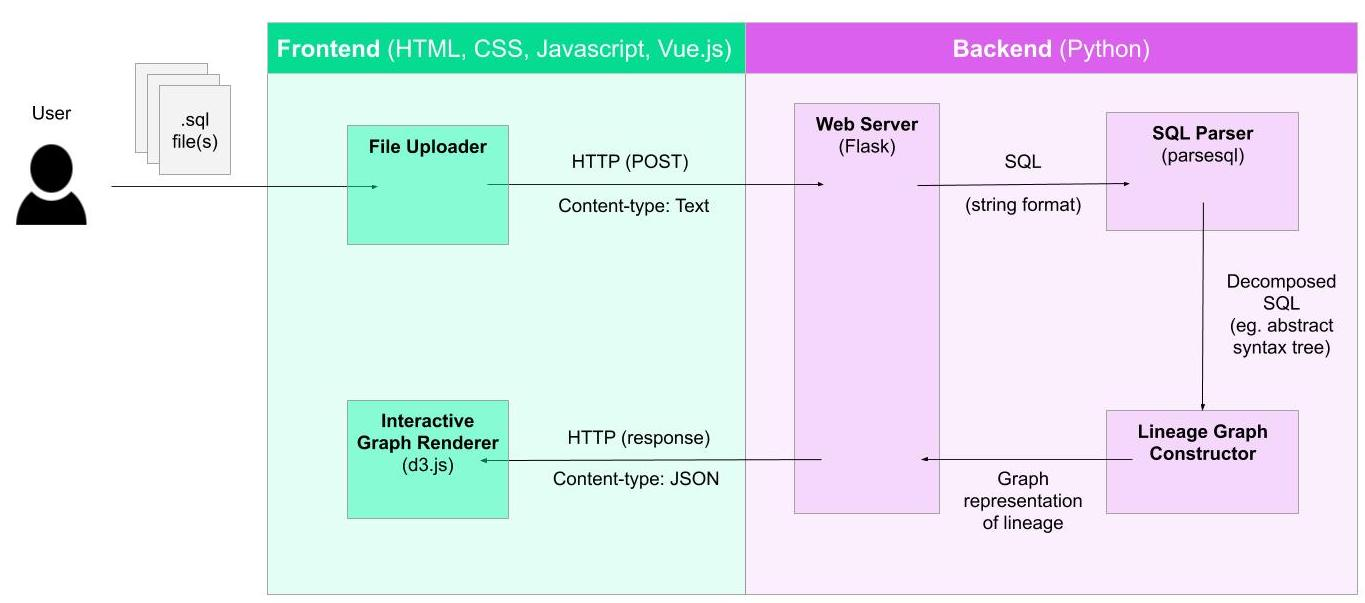
\includegraphics[width=\textwidth]{architecture.jpg}
  \label{fig:software-architecture-schematic}
\end{figure}

The architecture for the application seen in Figure \ref{fig:software-architecture-schematic} represents a Client-Server web application. A web application was selected based on the following considerations:

\begin{itemize}
\item Existence of relevant, open-source data visualisation libraries in JavaScript
\item Ability to implement back-end logic in Python (aligning with team member skills)
\item Maximise applications' availability - running through the web browser makes it independent of any particular operating system
\end{itemize}

The Client-Server model allows for separation of the SQL analysis logic from the visualisation components. This separation facilitates incremental development and increases modularity which is ideal for large, collaborative projects.\newline

For the average application usage, a user shall upload an sql file as input to the front-end File Uploader which will upload and convert the file content to string format. The file content shall be sent via HTTP POST to the Web Server which will forward the SQL content to a dedicated SQL Parser. In the back-end, the SQL Parser and Lineage Graph Constructor are responsible for decomposing the SQL input and formulating a programmatic representation of a graph containing the lineage relationships. This graph of lineage information shall be sent back to the front end in JSON format. The Interactive Graph Renderer shall take the lineage information and produce an interactive visual in the web browser. 
\end{spacing}